\documentclass[a4paper]{article}
\usepackage[utf8]{inputenc}
\usepackage[T1]{fontenc}
\usepackage[light,condensed,math]{kurier}
\usepackage[ngerman]{babel}
\usepackage{ntheorem}
\usepackage{graphicx}
\usepackage{floatrow}
\usepackage{float}
\usepackage{hyperref}

\theoremstyle{break}
\newtheorem{defi}{Definition}[section]
\newtheorem{ann}{Bemerkung}[section]
\newtheorem{der}{Folgerung}[section]
\newtheorem{ex}{Beispiel}[section]
\newtheorem{why}{Vorteile}[section]
\newtheorem{whynot}{Nachteile}[section]
\title{SWT 1: Solid Prinzipien}
\author{M. Goetze}

\begin{document}
	\maketitle
	\tableofcontents
	\newpage


\section{Single-responsibility principle}
\begin{defi}
	Eine Klasse hat genau eine Aufgabe. Eine Aufgabe bezeichnet hierbei einen 'Grund zur Änderung'
\end{defi}

\section{Open-closed principle}
\begin{defi}
	Software-Einheiten (Module, Klassen, Methoden etc.) sollen leicht erweiterbar sein, ohne dabei ihr Verhalten zu ändern.
\end{defi}

\section{Liskovsches Substitutionsprinzip}
\begin{defi}
	In einem Programm, in dem U eine Unterklasse von K ist, kann jedes Exemplar der Klasse K durch ein Exemplar von U ersetzt werden, wobei das Programm weiterhin korrekt funktioniert.
\end{defi}
\subsection{Vererbung}
\begin{defi}[Signaturvererbung]
Eine in der Oberklasse definierte (und evtl. implementierte) Methode überträgt nur ihre Signatur auf die Unterklasse.
\end{defi}

\begin{ann}
	In diesem Fall muss im UML-Klassendiagramm in der abgeleiteten Klasse die Methode erneut genannt werden.
\end{ann}

\begin{defi}[Implementierungsvererbung]
	Eine in der Oberklasse definierte und implementierte Methode überträgt ihre Signatur und ihre Implementierung auf die Unterklasse 
\end{defi}

\subsubsection{Varianz}
\begin{defi}[Kovarianz]
	Verwendung einer Spezialisierung des Parametertyps in der überschriebenen Methode
\end{defi}

\begin{defi}[Kontravarianz]
	Verwendung einer Verallgemeinerung des Parametertyps in der überschriebenen Methode.
\end{defi}

\begin{ann}
	Ferner existieren Varianz, Invarianz.
\end{ann}

\begin{ex}
	\begin{figure}[H]
		\centering
		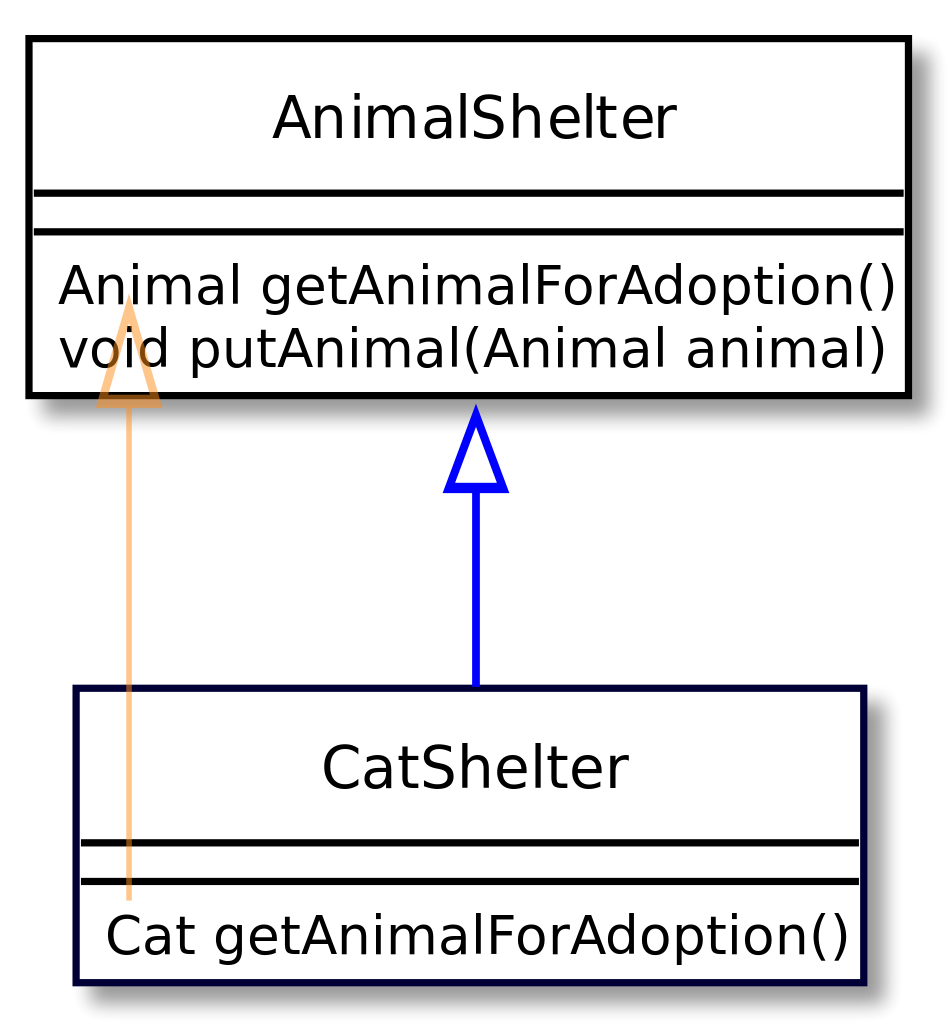
\includegraphics[width=\textwidth]{../diagrams/uml/covariance.png}
		\caption{Kovarianz des Rückgabetypen UML}
		\floatfoot{Source: (Vilhelm.s, Commons-Wiki, 26 July 2017)}
	\end{figure}
\end{ex}

\begin{ex}
	\begin{figure}[H]
		\centering
		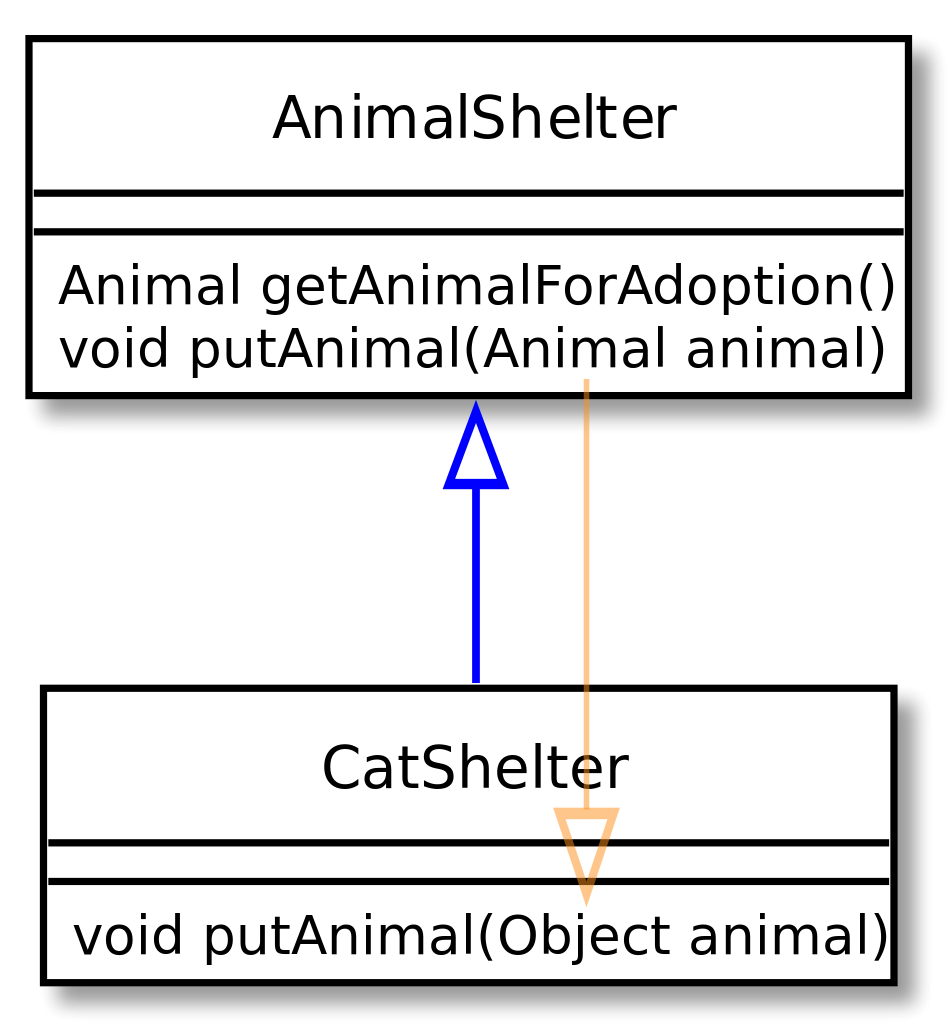
\includegraphics[width=\textwidth]{../diagrams/uml/contravariance.png}
		\caption{Kontravarianz der Parametertypen UML}
		\floatfoot{Source: (Vilhelm.s, Commons-Wiki, 26 July 2017)}
	\end{figure}
\end{ex}

\begin{der}
	Erlaubt für Eingabeparameter:
	\begin{itemize}
		\item Kontravarianz
		\item Invarianz
	\end{itemize}
	Erlaubt für Ausgabeparameter:
	\begin{itemize}
		\item Kovarianz
		\item Invarianz
	\end{itemize}
	Erlaubt für Parameter, die sowohl Ein- als auch Ausgabeparameter sind:
	\begin{itemize}
		\item Invarianz
	\end{itemize}
	Kontravarianz ist in Java nicht zulässig.
\end{der}

\subsubsection{Polymorphie}
\begin{defi}[dynamische Polymorphie]
	Es wird die Methode mit der angegebenen Signatur aufgerufen, die in der Vererbungshierarchie am speziellsten ist.
\end{defi}

\begin{ann}
	statische Polymorphie (Überladen: gleiche Signatur, unterschiedlicher Name) hat nichts mit Vererbung zu tun.
\end{ann}

\section{Interface-Segregation-Prinzip}
\begin{defi}
	Interfaces sollten nichts weiter können, als das, was ein Klient konkret benötigt.
\end{defi}
\begin{der}
	Aufteilung von Software in entkoppelte Klassen. 
\end{der}

\section{Dependency-Inversion-Prinzip}
\begin{defi}
	Abhängigkeiten von konkreten Modulen niedriger Ebene sollten aussschließlich zu abstrakten Modulen höherer Ebene gerichtet sein.
\end{defi}

	
\end{document}